\section{Experiment}
%Give artists the task to make a video in a certain scene using some specific features, both in Unity and in Maya. We can then compare their performances, and if the two performances are significantly close, the tool was a success.

%Video and audio recordings. Time spent on tasks. Few questions about usability and experience.

%(Hypotheses - not sure yet?)

(This is obviously not done yet)

\subsection{Purpose of the test}
\begin{enumerate}
\item To find out if the FEELS tea's mental models of the camera system match how the system actually works.
\item Compare other artists from TAW 3rd year using the camera system with the FEELS team.
\end{enumerate}


%Figure \ref{fig:test_overview} shows the criteria for the two testing groups \footnote{This will not be in the final paper; it's just for helping you to understand what we mean.}


%\begin{figure}[htbp]
%\centering
%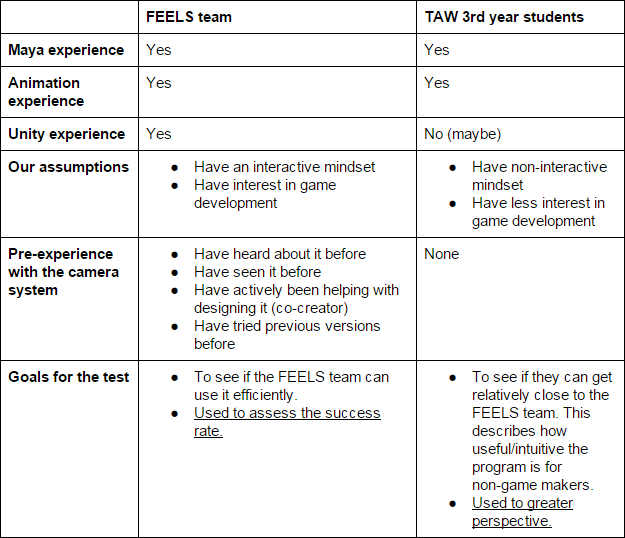
\includegraphics[width=0.5\textwidth]{Pics/test_table_temp}
%\caption{Overview of the testing groups.}
%\label{fig:test_overview}
%\end{figure}

\subsection{The Three Phases of the Experiment}
\textbf{PHASE 1 - Training:}
\begin{enumerate}
\item Place framings along the movement path so that there's at least one framing in "move path section".
\item Tell the facilitator about the functionality of each button in the interface as you think it'll work.
\item Split a framing connection into two.
\item Delete a framing.
\end{enumerate}

Specific tasks:
\begin{enumerate}
\item Make the camera's field of view change when player gets close to it
\item Make the camera tilt upwards when player gets close to it
\item Make the camera pan to the left when player gets close to it
\item Make the camera look at object X when the player gets close to it
\item Make the camera dolly away from the character as the player walks along a path.
\item Make the camera look from the ground upwards
\item Change the interpolation of one of the previous assignments by changing the animation curve.
\end{enumerate}

\textbf{PHASE 2 - Re-create camera:}
\begin{itemize}
\item Show a video of the end result
\item Recreate this as closely as possible?
\end{itemize}

\textbf{PHASE 3 - Be creative:}
\begin{itemize}
\item Give them environment with path already there, do what you want. Test the limits of the system.
\end{itemize}
